% Für Bindekorrektur als optionales Argument "BCORfaktormitmaßeinheit", dann
% sieht auch Option "twoside" vernünftig aus
% Näheres zu "scrartcl" bzw. "scrreprt" und "scrbook" siehe KOMA-Skript Doku
\documentclass[12pt,a4paper,titlepage,headinclude]{scrartcl}

%%%%%%%%%%%%%%%%%%%%%%%%%%%%%% Formatierung %%%%%%%%%%%%%%%%%%%%%%%%%%%

%keine Einrückung nach leerzeile
\parindent0pt

% Für Kopf und Fußzeilen, siehe auch KOMA-Skript Doku
\usepackage[komastyle]{scrpage2}
\pagestyle{scrheadings}
\setheadsepline{0.5pt}[\color{black}]
\automark[section]{chapter}

%Zitate und Literaturverzeichnis
\usepackage[backend=bibtex,natbib=true,sorting=nyt,style=numeric-comp]{biblatex}
\usepackage[babel,german=quotes]{csquotes}
\bibliography{literatur}

%Zur vernünftigen Dekodierung
\usepackage[T1]{fontenc} %
\usepackage[utf8]{inputenc} %utfx8
\usepackage[ngerman]{babel} %

%Interaktives Dokument
\usepackage[pdfpagelabels=true]{hyperref}%

%Für wissenschaftliches Zitieren
%\usepackage{natbib}

%Schriftarten
%\usepackage{lmodern} %

%Formatierung für Kof- und Fußzeile. Hier gilt entweder ... oder ...!!

%Für eigenen Zeilenabstand
\usepackage{setspace} %

%Für die Seitenformatierung
\usepackage{lscape} %
\usepackage{multicol} %
\usepackage{wallpaper} %

%Styling Inhaltsverzeichnis
\usepackage{tocloft} %

% Zur Formatierung für Kopf und Fußzeilen. Im Allgemeinen ist scrpage2 besser als fancyhdr
\usepackage{scrpage2}
\pagestyle{scrheadings}
\setheadsepline{0.5pt}[\color{black}]

%Einstellungen für Figuren- und Tabellenbeschriftungen
\setkomafont{captionlabel}{\sffamily\bfseries}
\setcapindent{0em} 


%%%%%%%%%%%%%%%%%%%%%%%%%%%%%% Mathematisches %%%%%%%%%%%%%%%%%%%%%%%%%%%

%Pakete für Mathesymbole
\usepackage{latexsym,exscale,stmaryrd} %
\usepackage{amssymb, amsfonts, amstext} %
\usepackage{amsmath, mathtools, amsthm} %

%align nummerierung
\numberwithin{equation}{subsection}

% Weitere Symbole
\usepackage[nointegrals]{wasysym} %
\usepackage{eurosym} %
\usepackage{textcomp} %

%\usepackage{ucs} %

%Für vernünftige Einheiten 
\usepackage[separate-uncertainty, exponent-product = \cdot]{siunitx}
%\usepackage[thinspace,thinqspace,amssymb]{SIunits} %
\usepackage{icomma} %
\usepackage{nicefrac}%

%SI-Einheiten
\usepackage{siunitx}

%%%%%%%%%%%%%%%%%%%%%%%%%%%%%% Grafiken & Tabellen %%%%%%%%%%%%%%%%%%%%%%%%%%%
% Text umfließt Graphiken und Tabellen
% Beispiel:
% \begin{wrapfigure}[Zeilenanzahl]{"l" oder "r"}{breite}
%   \centering
%   \includegraphics[width=...]{grafik}
%   \caption{Beschriftung} 
%   \label{fig:grafik}
% \end{wrapfigure}
% Mehrere Abbildungen nebeneinander
% Beispiel:
% \begin{figure}[htb]
%   \centering
%   \subfigure[Beschriftung 1\label{fig:label1}]
%   {\includegraphics[width=0.49\textwidth]{grafik1}}
%   \hfill
%   \subfigure[Beschriftung 2\label{fig:label2}]
%   {\includegraphics[width=0.49\textwidth]{grafik2}}
%   \caption{Beschriftung allgemein}
%   \label{fig:label-gesamt}
% \end{figure}

%Subfigure nur mit PDF statt Bildern einfügen:
\usepackage{adjustbox}
%\begin{figure}[h]
%  \centering
%  \subfigure[Caption1\label{fig:bild1}]
%  {\begin{adjustbox}{width=0.44\linewidth}\input{bild1}\end{adjustbox}}
%  \hfill
%  \subfigure[Caption2\label{bild2}]
%  {\begin{adjustbox}{width=0.44\linewidth}\input{bild2}\end{adjustbox}}
%  \hfill
%  \subfigure[Caption3\label{bild3}]
%  {\begin{adjustbox}{width=0.44\linewidth}\input{bild3}\end{adjustbox}}
%  \caption{Gesamtcaption}
%  \label{fig:gesamtlabel}
%\end{figure}

%\usepackage{subfigure}




% Caption neben Abbildung
% Beispiel:
% \sidecaptionvpos{figure}{"c" oder "t" oder "b"}
% \begin{SCfigure}[rel. Breite (normalerweise = 1)][hbt]
%   \centering
%   \includegraphics[width=0.5\textwidth]{grafik.png}
%   \caption{Beschreibung}
%   \label{fig:}
% \end{SCfigure}

%Einstellungen für Figuren- und Tabellenbeschriftungen
\setkomafont{captionlabel}{\sffamily\bfseries}
\setcapindent{0em}

%Fuer mehr Platz in den Tabellen
\usepackage{cellspace} %mehr Platz in Tabellen
\addtolength\cellspacetoplimit{3pt}
\newcommand\myhline[1][2pt]{\\[#1]\hline}

%Zum Einbinden von GRafiken
\usepackage{graphicx}% [pdflatex]
\usepackage{xcolor}%

%Für textumflossene Grafiken
\usepackage{wrapfig} %

%Für subfigure
\usepackage{caption}
\usepackage{subcaption}

% Caption neben Abbildung
\usepackage{sidecap}

%Für URLs
\usepackage{url}%

%Zum Einbinden von Quelltext
\usepackage{listings-ext} %

%Für chemische Formeln
\usepackage{chemfig} %
%Für chemische Formeln (von www.dante.de)
%% Anpassung an LaTeX(2e) von Bernd Raichle
\makeatletter
\DeclareRobustCommand{\chemical}[1]{%
  {\(\m@th
   \edef\resetfontdimens{\noexpand\)%
       \fontdimen16\textfont2=\the\fontdimen16\textfont2
       \fontdimen17\textfont2=\the\fontdimen17\textfont2\relax}%
   \fontdimen16\textfont2=2.7pt \fontdimen17\textfont2=2.7pt
   \mathrm{#1}%
   \resetfontdimens}}
\makeatother
%erzwinge Fussnote auf selber Seite
\interfootnotelinepenalty=1000

%Zusätzliche Boxen
\usepackage{fancybox}

%\usepackage{framed}
%\usepackage{mathmode}
%\usepackage{empheq}

%Für variable Referenzen
\usepackage{varioref}

%Für Tabellen mit fester Gesamtbreite und variabler Spaltenbreite (im Gegensatz zu tabular)
\usepackage{tabularx}
%\newcommand{\ltab}{\raggedright\arraybackslash} % Tabellenabschnitt linksbündig
%\newcommand{\ctab}{\centering\arraybackslash} % Tabellenabschnitt zentriert
%\newcommand{\rtab}{\raggedleft\arraybackslash} % Tabellenabschnitt rechtsbündig


%Für Gleitobjekte
\usepackage{float} %Für H-Option

\usepackage{multirow} % Zellen von Tabellen zusammenfassen
\usepackage{booktabs} % verschoenert Tabellen
\usepackage{fixltx2e} % Repariert einige Dinge in Bezug auf das setzen von Gleitobjekten http://ctan.org/pkg/fixltx2e
\usepackage{stfloats} % Bei Gleitobjekten (figure,table,...) die ueber zwei Spalten gesetzt werden (Umgebung figure*), funktioniert [tb] http://ctan.org/pkg/stfloats
\usepackage{rotating} % Wird für Text und Grafiken benötigt, die um einen Winkel gedreht werden sollen



%%%%%%%%%%%%%%%%%%%%%%%%%%%%%% Kommandodefinitionen %%%%%%%%%%%%%%%%%%%%%%%%%%%

%Zur Korrektur und Kommentierung
\newcommand{\comment}[1]{\marginpar{\tiny{\textcolor{red}{#1}}}} % ermoeglicht kleine Kommentare am Seitenrand: \comment{Fehler?}
\newcommand{\Comment}[1]{\textcolor{red}{#1}}

%Zur Formatierung in der Matheumgebung
\renewcommand{\t}{\ensuremath{\rm\tiny}} % Tiefgestellter Text in der Matheumgebung wird schoener mit: $\Phi_{\t{Text}}$
\renewcommand{\d}{\ensuremath{\mathrm{d}}} % Die totale Ableitung ist stets aufrecht zu setzen: \d
\newcommand{\diff}[3][]{\ensuremath{\frac{\d^{#1}#2}{\d#3^{#1}}}} % einfache Ableitung nach x: $\ddx{\Phi}$
\newcommand{\pdiff}[3][]{\ensuremath{\frac{\partial^{#1}#2}{\partial#3^{#1}}}} % wie gesprochen, eine partielle Ableitung: \del
\newcommand{\aeqiv}{\ensuremath{\qquad \Longleftrightarrow \qquad}} % Eine Aequivalenz
\newcommand{\folgt}{\ensuremath{\qquad \Longrightarrow \qquad}} % Ein Folgepfeil mit Abstaenden
\newcommand{\corresponds}{\ensuremath{\mathrel{\widehat{=}}}} % Befehl für "Entspricht"-Zeichen
\newcommand{\mi}[1]{\ensuremath{\mathit{#1}}} % italics für griechische Buchstaben in Matheumgebung

%Um nicht so viel schreiben zu müssen...
\newcommand{\bs}[1]{\boldsymbol{#1}}
\newcommand{\ol}[1]{\overline{#1}}
\newcommand{\wtilde}[1]{\widetilde{#1}}
\newcommand{\mrm}[1]{\mathrm{#1}}
\newcommand{\mbf}[1]{\mathbf{#1}}
\newcommand{\mbb}[1]{\mathbb{#1}}
\newcommand{\mcal}[1]{\mathcal{#1}}
\newcommand{\mfrak}[1]{\mathfrak{#1}}

%Abkürzungen
\newcommand{\zB}{z.\,B.\ }
\newcommand{\bzw}{b.\,z.\, w.\ }
\newcommand{\Dh}{d.\,h.\ }
\newcommand{\Gl}{Gl.\ }
\newcommand{\Abb}{Abb.\ }
\newcommand{\Tab}{Tab.\ }

%Farbige Box um eine Formel
%Anwendung:
%\eqbox{
%  \begin{equation}
%    ...
%  \end{equation}
%}
\newcommand{\eqbox}[1]{
  \colorbox{gray!30}{\parbox{\linewidth}{#1}} 
}

%Im Text
\newcommand{\engl}[1]{engl. \textit{#1}}
\newcommand{\zitat}[1]{\footnote{#1}}
\newcommand{\person}[1]{\textsc{#1}}


%Matheoperatoren
\DeclareMathOperator{\tr}{tr}
\DeclareMathOperator{\sgn}{sgn}
\DeclareMathOperator{\diag}{diag}
\DeclareMathOperator{\const}{const}
\DeclareMathOperator{\grad}{grad}
\DeclareMathOperator{\rot}{rot}
\DeclareMathOperator{\divz}{div}


%%%%%%%%%%%%%%%%%%%%%%%%% Quellcode - Formatierung %%%%%%%%%%%%%%%%%%%%%%%%%%%%%%%%%%%%%%

%Um auch Umlaute in den Kommentaren auswerten zu können
\lstset{
literate = {Ö}{{\"O}}1 {Ä}{{\"A}}1 {Ü}{{\"U}}1 {ß}{{\ss}}2 {ü}{{\"u}}1
           {ä}{{\"a}}1 {ö}{{\"o}}1
}

%Formatierung des Quellcode
\lstset{
language=C++,
basicstyle=\footnotesize\ttfamily,
keywordstyle=\bfseries\color{blue},
stringstyle=\color{red},
commentstyle=\itshape\color{green!60!black},
emphstyle = \bfseries\color{red!80!green!60!blue}
%identifierstyle=,
}

%Zum Hervorheben bestimmter Begriffe (z.B. eigene Klassen, etc.)
%\lstset{
%emph = {vector, iterator, std, ostream, istream , ofstream, ifstream, fstream, cmath}
%}

%Nummerirung
\lstset{
numbers=left,
numberstyle=\tiny,
stepnumber=2,
numbersep=5pt,
frame=single,
breaklines=true
framesep=5pt,
numbersep=8pt,
breakindent=3ex
}

%Einbunden über
%\lstinputlisting[caption={blablabla}, language=C++]{name.cpp}

\begin{document}
%Autor, etc.
\newcommand{\versuch}{Versuch 18}
\newcommand{\titel}{Mikroskop}
\newcommand{\praktikantA}{Eric Bertok}
\newcommand{\praktikantB}{Kevin Lüdemann}
\newcommand{\betreuer}{Phillip Bastian}
\newcommand{\emailA}{
      \href{mailto:eric.bertok@stud.uni-goettingen.de }
           {eric.bertok@stud.uni-goettingen.de} }
\newcommand{\emailB}{
      \href{mailto:kevin.luedemann@stud.uni-goettingen.de}
           {kevin.luedemann@stud.uni-goettingen.de} }
\newcommand{\gruppe}{B001}
\newcommand{\durchfuehrungsdatum}{04.03.2014}
\newcommand{\abgabedatum}{05.03.2014}

%Metainformationen
\hypersetup{
      pdfauthor = {\praktikantA~ },
      pdftitle  = {\versuch: \titel},
      pdfsubject = {\titel}
}

\begin{titlepage}
\centering
\textsc{\Large Anfängerpraktikum der Fakultät für
  Physik,\\[1.5ex] Universität Göttingen}

\vspace*{2.5cm}

\rule{\textwidth}{1pt}\\[0.5cm]
{\huge \bfseries
  \versuch\\[1.5ex]
  \titel}\\[0.5cm]
\rule{\textwidth}{1pt}

\vspace*{2.5cm}

\begin{Large}
\begin{tabular}{ll}
Praktikanten: &  \praktikantA,\\
	      &  \praktikantB \\
Email:	& \emailA\\
	& \emailB\\
Gruppe: & \gruppe\\
Betreuer: & \betreuer\\
Durchgeführt am: & \durchfuehrungsdatum\\
Abgegeben am: & \abgabedatum\\
\end{tabular}
\end{Large}
\vspace*{0.8cm}

\begin{Large}
\fbox{
  \begin{minipage}[t][2.5cm][t]{6cm} 
    Testat:
  \end{minipage}
}
\end{Large}

\end{titlepage}

\cleardoublepage
\tableofcontents
\thispagestyle{empty}
\cleardoublepage

\setcounter{footnote}{0}
\setcounter{page}{1}

\pagenumbering{arabic}

\newpage

\section{Einleitung}
\label{sec:einleitung}
Das Mikroskop ist seit vielen Jahrhunderten das wichtigste Messinstrument, wenn es darum geht, kleine Objekte zu betrachten.
Der schematische Aufbau existiert bereits seit 1673 und wurde von Anton Leuvenhook gebaut.
Heutzutage verwendet man es immer noch, z.B. in der Medizin.
Aus diesem Grund beschäftigt sich dieser Versuch mit den Grundlegenden Eingenschaften, wie der Vergrößerung und dem Auflösungsvermögen eines Mikroskops.

\section{Theorie}
\label{sec:theorie}

\subsection{Strahlenoptik}
Die Strahlenoptik beschreibt die Ausbreitung von Licht als Strahlen, welche sich im Vakuum als Geraden ausbreiten.
Diese können mithilfe von Grenzflächen gebrochen und reflektiert werden.
Eine Möglichleit die Strahlen zu beeinflussen sind Linsen.

\subsubsection{Linsen}
Es gibt zwei Arten von Linsen: Sammel- und Zerstreuungslinsen.
Die Sammellinsen sind konvex oder konvex-plan geformt und haben bei parallel eintreffendem Licht einen Brennpunkt, in dem alle Strahlen gebündelt werden.
Dies gilt auch für schräg einfallendes Licht, hier müssen aber verschiedene Abbildungsfehler beachtet werden.\\
Die Zertstreuungslinsen sind konkav oder konkav-plan geformt und haben keinen Punkt, in dem sie das einfallende, parallele Licht bündeln.
Dieser Linsentyp defokussiert, also zerstreut die Strahlen.
Dies gilt auch wieder für schräg einfallendes Licht, aber auch hier muss wieder mit erheblichen Abbildungsfehlern gerechnet werden.
Zur Berechnung der Fokuslänge wird die \person{Gaus}abildungsformel verwendet \cite[279]{demtroeder2} 
\begin{align}
	\frac{1}{f}=\frac{1}{b}+\frac{1}{g}.\label{eq:gaus}
\end{align}
Für die Vergrößerung gilt nach \cite[280]{demtroeder2}
\begin{align}
	V=\frac{B}{G}=\frac{b}{g}.\label{eq:vergr}
\end{align}

\subsubsection{Brechung}
Trifft ein Lichtstrahl auf eine Grenzfläche, bei der der Brechungsindex veschieden vom vorherigen Medium ist, so wird der Lichtstrahl entweder reflektiert oder gebrochen.
Diese beiden Fälle sind nur im Spezialfall getrennt, denn normalerweise treten beide Effekte auf, haben aber unterschiedliche Intensitäten.
Bei der Brechung wird der auslaufende Strahl über den Einfallswinkel und den Quotienten der Brechungsindizes bestimmt.
Es gilt das Snelliussche Brechunggesetz \cite[101]{hecht}:
\begin{align}
	\sin{\theta_1}=\frac{n_1}{n_2}\sin{\theta_2}.
\label{eq:snell}
\end{align}


\subsection{Auflösungsvermögen}
Das Auflösungsvermögen ist über das Rayleigh-Kriterium \cite[366]{demtroeder2} definiert.
Zwei Punkte nicht mehr auflösen zu können bedeutet, dass man beide nicht mehr voneinander unterscheiden kann.
Der minimale Abstand dieser Punkte, bzw. der minimale Winkelabstand ist definiert als
\begin{align}
	\sin{\delta}_\text{min}=1.22\frac{\lambda}{b},\label{eq:rayleight}
\end{align}
wobei $\lambda$ die Wellenlänge ist und $b$ der Abstand vom Objekt zum Objektiv.
Für ein Mikroskop ist die minimal noch auflösbare Länge somit
\begin{align}
	x_\text{min}=\frac{\lambda}{N},\label{eq:aufloes}
\end{align}
wobei $x_\text{min}$ der minimale Abstand zwischen zwei Punten ist, damit sie getrennt aufgelöst werden können, und $N$ die Numerische Aperatur.
Das Auflösungsvermögen ist definiert als der Kehrwert der Länge $x_min$.
Die Numersiche Apperatur ist eine Kenngröße für das Auflösungsvermögen eines Mikroskops, welche gegeben ist durch das Produkt aus Brechzahl $n$ und des Sinuses des Winkels zwischen optischer Achse und Randpunkt des Lichtkegels \cite[369]{demtroeder2}:
\begin{align}
	N=n\cdot\sin{\alpha}.\label{eq:numapp}
\end{align}

\subsection{Mikroskop}
Ein Mikroskop ist ähnlich zu einem Fernrohr, wobei das Objekt nicht im unendlichen steht.
\begin{figure}[!h]
\centering
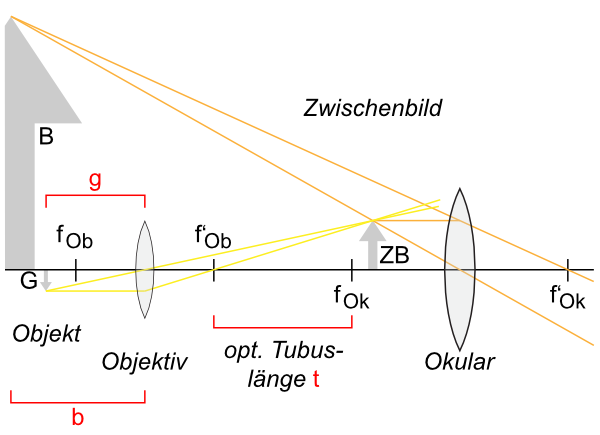
\includegraphics{mikroskop.png}
\caption{Linsensystem eines Mikroskops. Das Objekt erzeugt ein reelles Zwischenbild, welches dann durch die zweite Linse ein virtuelles Bild erzeugt. Die zweite Linse wirkt wie eine Lupe, da das Zwischenbild hinter dem Fokus der Linse liegt. \cite[Abgerufen am: 04.03.2015]{LP17}}
\label{fig:linsenmikroskop}
\end{figure}
In der Graphik \ref{fig:linsenmikroskop} ist das Linsensystem eines Mikroskops zu sehen.
Das Objekt erzeugt durch die erste Linse ein reelles Zwischenbild.
Dieses wird dann mithilfe der zweiten Linse auf ein virtuelles Bild abgebildet.
Die zweite Linse wirkt wie eine Lupe und vergrößert das Zwischenbild noch einmal.
Die Tubuslänge ist der Abstand zwischen den Fokuspunkten der beiden Linsen
Die Gesamtvergrößerung errechnet sich aus dem Produkt der beiden Vergrößerungen:
\begin{align}
	V_\text{ges}=V_\text{Objektiv}\cdot V_\text{Okular}.
\end{align}
Aus den Formeln \eqref{eq:vergr} und \eqref{eq:gaus} lässt sich die Vergrößerung des Objektivs und Okulars berechnen.
Die Differenz der beiden ergibt dann eine Gleichung über die Differenz in der Tubuslänge $\Delta t$:
\begin{align}
	V_\text{lang}-V_\text{kurz}=\frac{t_\text{lang}}{f}-\frac{t_\text{kurz}}{f}=\frac{\Delta t}{f}.\label{eq:f}
\end{align}

\section{Durchführung}
\label{sec:durchfuehrung}

\subsection{Mikroskop}
Das Mikroskop hat zwei Okulare, ein senkrechtes und ein gekipptes.
Zudem werden zwei verschiedenen Objektive verwendet, eins mit 10 facher und mit 40 facher Vergrößerung.
Im gekippten Okular befindet sich ein kurzer, verschiebbarer Tubus mit einer Matscheibe.
Auf dieser wird das Zwischenbild abgebildet.
Als Objekt wird ein Objektträger mit Skala verwendet.\\
Für den ersten Teil des Versuches wird je drei mal die Skala mit beiden Vergrößerungen fokussiert und mit einem parallel zur Objektskala liegenden Maßtab vermessen.
Dazu wird die Skala fokussiert und über das zweite Auge mit der anderen Skala in Deckung gebracht.
Hier kann jetzt die Größe des Objektes gemessen werden.\\
Für den zweiten Teil wird nun die fokussierte Skala auf der Mattscheibe abgebildet und vermessen.
Dies wird ebenfalls drei mal durchgeführt.
Es bietet sich an diesen Teil des Versuches mit dem ersten zusammen durchzuführen.\\
Im dritten Teil wird der kurze sowie lange Tubus, welcher ganz im gekippten Okular steckt, verwendet.
Diesmal wird das Zwischenbild fokussiert ohne den Tubus in der Länge zu verändern.
Wieder wird die Größe des Zwischenbildes vermessen.\\
Um die Auswertung zu vereinfachen ist es möglich, immer die gleiche Skalenlänge zu vermessen.

\subsection{Optische Schiene}
In diesem Teil des Versuches wird eine optische Schiene mit einer Lampe, einem Farbfilter von 650 \si{\nano\meter}, einem Glasmastab, einem Spalt mit veränderbarer Breite und einem Tubus verwendet.
Der Spalt wird dierekt vor den Tubus gestellt und ganz geöffnet.
Anschließend wird der Glasmastab fokussiert und der Spalt soweit geschlossen, bis der Masstab nicht mehr aufgelöst werden kann.
Es ist jetzt der Abstand zwischen Maßtab und Spalt zu messen.\\
Jetzt wird der Maßtab entfernt, der Spalt fokussiert und der Abstand zwischen dem Spalt vorher und nachher gemessen.
Dies wird einfacher, wenn der Spalt vorher dierekt am Tubus liegt.
Anschließend wird mit dem Mikrometertrieb und dem Fadenkreuz die Spaltbreite vermessen.
Wichtig ist noch die Vergrößerung des Mikroskopes zu notieren.\\
Im letzten Teil wird auch der Spalt entfernt und der Plexiglasstab eingebaut, sodass die Skala in Richtung der Lichtquelle zeigt.
Der Stab wird auf der Vorderseite fokussiert und anschließend das Okular gegen eine Lochblende eingetauscht, die ganz in den Tubus geschoben wird.
Mit diesem Aufbau kann die Anzahl der Skalenteile gezählt werden.
Für diese Skala gilt ein Abstand der Skalenteile von 0.5 \si{\milli\meter}.
Es ist hilfreich die Tischlampe so einzustellen, dass sie den Stab seitlich beleuchtet.

\section{Auswertung}
\label{sec:auswertung}
\subsection{Bestimmung der Okularvergrößerung}
Zunächst werden aus den verschiedenen Messungen aus Durchführungspunkt 1 und 2 der Mittelwert und die Standardabweichung bestimmt. Als systematische Ungenauigkeit wird für das 10$\times$-Objetktiv für die Längenmessung durch das Okular $\sigma_{B_{10\times}}=\SI{1}{\milli\metre}$ und für das 40$\times$-Objektiv der Doppelte Fehler von $\sigma_{B_{40\times}}=\SI{2}{\milli\metre}$ verwendet. Ersterer ist die kleinstmögliche Skaleneinteilung des Vergleichsmasßstabes. Bei dem 40$\times$-Objektiv ist die Ungenauigkeit größer, da die Skalenstriche des eingespannten Maßstabes breiter waren, als die Genauigkeit des Vergleichsmaßstabes. Die Standardabweichung der Mittelwerte werden zu den systematischen Fehlern hinzuaddiert. Die fehlerbehafteten Mittelwerte sind in Tabelle \ref{tab:mess1} zusammengetragen.
Eine Skala des zu messenden Maßstabs ist $\SI{0.5}{\milli\metre}$ lang.
\begin{table}[H]
	\centering
	\begin{tabular}{|c|c|c|c|}\hline
		Objektiv&Skalen $N$&Größe durch Okular $B_{o}$\;[mm]&Zwischengröße $B_z$\;[mm]\\\hline
		10$\times$&2&$101.3\pm1.6$&$9.53\pm0.16$\\\hline
		40$\times$&0.5&$100.7\pm1.6$&$9.42\pm0.6$\\\hline	

	\end{tabular}
	\caption{Mittelwerte des 1. und 2. Durchführungsteils.}
	\label{tab:mess1}
\end{table}
Die Gesamtvergrößerung $V$ ergibt sich nach Gl. \eqref{eq:vergr}
\begin{align}
	V=\frac{B_o}{G}
\end{align}
Der Fehler berechnet sich nach der \person{Gauss}schen Fehlerfortpflanzungsformel zu
\begin{align}
	\sigma_V=|\frac{\sigma_{B_o}}{G}|.
	\label{eq:sigV}
\end{align}
Für die Okularvergrößerung $V_\text{ok}$ muss noch analog zur Gesamtvergrößerung die Vergrößerung durch das Objektiv $V_\text{obj}$ nach
\begin{align}
	V_\text{obj}=\frac{B_z}{G}
\end{align}
berechnet werden. Anschließend erhält man die Okularvergrößerung nach
\begin{align}
	V_\text{ok}&=\frac{V}{V_\text{obj}},\\
	\sigma_{V_\text{ok}}&=\sqrt{\frac{\sigma_V^2}{V_\text{obj}^2}+\frac{\sigma_{V_\text{obj}}^2\cdot V^2}{V_\text{obj}^4}}
	\label{eq:Vok}
\end{align}
Die Endergebnisse sind in Tabelle \ref{tab:erg1} zu sehen.
\begin{table}[H]
	\centering
	\begin{tabular}{|c|c|c|c|}
		\hline
		Objektiv&Gesamtvergr. $V$&Objektivvergr. $V_\text{obj}$&Okularvergr. $V_\text{ok}$\\\hline
		$10\times$&$101.3\pm1.6$&$9.53\pm0.16$&$10.63\pm0.3$\\\hline
		$40\times$&$403\pm7$&$38\pm3$&$10.7\pm0.7$\\\hline
	\end{tabular}
	\caption{Endergebnisse des 1. und 2. Auswertungsteils.}
	\label{tab:erg1}
\end{table}
Als gewichteter Mittelwert für die Okularvergrößerung erhält man
	\begin{equation}
		\overline{V}_\text{ok}=10.6\pm0.3
		\label{eq:mittelok}
	\end{equation}
\subsection{Bestimmung der Brennweite der Objektive}
Zunächst werden wieder die gemessenen Daten gemittelt. Sie sind in Tabelle \ref{tab:Mittel2} zu sehen. Anschließend kann gemäß Gleichung \eqref{eq:f} aus den zwei Objektivvergrößerungen $V_{\text{lang}}$ und $V_\text{kurz}$ die Brennweite $f$ der Objektive bestimmt werden:
	\begin{align}
		f&=\frac{\Delta t}{\Delta V}=\frac{\Delta t}{V_\text{lang}-V_\text{kurz}},\\
		\sigma_f&=\sqrt{\frac{(\sigma_{V_\text{lang}}^2+\sigma_{V_\text{kurz}}^2)\cdot\Delta t^2}{(V_{\text{lang}}-V_\text{kurz})^4}+\frac{\sigma_{\Delta t}^2}{(V_{\text{lang}}-V_\text{kurz})^2}}
		\label{eq:fumgestellt}
	\end{align}
	\begin{table}
		\centering
		\begin{tabular}{|c|c|c|c|c|}
			\hline
			Objektiv&$B_\text{kurz} [\text{mm}]$&$B_\text{lang} [\text{mm}]$&$V_\text{kurz}$&$V_\text{lang}$\\\hline
			10$\times$&$8.73\pm0.06$&$12.93\pm0.06$&$8.73\pm0.06$&$12.93\pm0.06$\\\hline
			40$\times$&$8.90\pm0.06$&$12.70\pm0.06$&$35.6\pm0.24$&$50.8\pm0.24$\\\hline
		\end{tabular}
		\caption{Mittelwerte der Messwerte und berechnete Objektivvergrößerungen für die beiden Tubuslängen.}
		\label{tab:Mittel2}
	\end{table}
	Für die Differenz der Tubuslängen $\Delta t$ beträgt der Mittelwert $\Delta t=(81.6\pm0.06)\,\text{mm}$.
	Auch für diese Messung wurde eine Ungenauigkeit von $\sigma_{\Delta t}=\SI{0.1}{\milli\metre}$ angenommen, also die Genauigkeit des Messschiebers. 
	Die Ergebnisse aus den Gleichungen \eqref{eq:fumgestellt} sind in Tabelle \ref{tab:f} zusammengetragen.
	\begin{table}[H]
		\centering
		\begin{tabular}{c}
			$f_{10\times}=(19.4\pm0.4)\,$mm\\
			$f_{40\times}=(5.4\pm0.2)\,$mm
		\end{tabular}
		\caption{Endergebnisse für die Brennweiten der beiden Objektive}
		\label{tab:f}
	\end{table}
	

\subsection{Optische Schiene}
\begin{figure}[!h]
\centering
\resizebox{\textwidth}{!}{\input{schieneStrahlengang.pdf_tex}}
\caption{Strahlengang der optischen Schiene mit Glasmasstab und Spalt. Quelle: http://www.genug-davon.de/aprakt/index.php?section=v18, abgerufen am 04.03.2015}
\label{fig:strahl1}
\end{figure}
Der Strahlengang des Aufbaus mit der Glasmesskala und dem Spalt ist in Abbildung \ref{fig:strahl1} zu sehen.
Die beiden Lichtpunkte in der Abbildung stellen zwei verschiedene Punkte auf der Glasmesskala da.
Diese Beiden werden durch den Spalt beschränkt und schließlich im Okular wieder gebündelt.\\
\begin{figure}[!h]
\centering
\resizebox{\textwidth}{!}{\input{strahlengang3.pdf_tex}}
\caption{Strahlengang der optischen Schiene mit dem Plexiglasstab und der Lochblende. Quelle: http://www.genug-davon.de/aprakt/index.php?section=v18, abgerufen am 04.04.2015}
\label{fig:strahl2}
\end{figure}
Der Strahlengang des Aufbaus mit dem Plexiglasstab und der Lochblende ist in der Abbildung \ref{fig:strahl2} zu sehen.
Der Abstand $d$ ist der Abstand zwischen den Skalenteilen auf dem Stab von denen aus die Strahlen durch das Objektiv und die Lochblende abgebildet.\\\\
Die Skala des Glasmasstab ist bei 1/10 \si{\milli\meter}, somit ist der Abstand zwischen zwei Skalenteilen $s=0.1\si{\milli\meter}$.
Die Spaltbreite ist so klein eingestellt, dass der Abstand zwischen zwei Skalenteilen nicht mehr aufgelöst werden kann, also ist $s=x_\text{min}$.
Das theoretische Auflösungsvermögen ist nach \eqref{eq:aufloes} $A=s^{-1}=10\;\text{mm}^{-1}$.\\\\
Mithilfe des Mikrometertriebes wurde eine Spaltbreite von $d=0.78\pm0.1\si{\milli\meter}$ gemessen, wobei der Fehler mit $0.1\si{\milli\meter}$ abgeschätzt wurde.
Für den Abstand zwischen Spalt und Objektiv wurde eine Länge von $L=47.0\pm0.1\si{\milli\meter}$ gemessen, wobei der Fehler mit $0.1\si{\milli\meter}$ abgeschätzt wurde.
Aus dem Strahlengang in Abbildung \ref{fig:strahl1} kann der Sinus geschrieben werden als
\begin{align}
	\sin{\alpha}&=\frac{d}{L}=0.017\pm0.003  \text{ mit,}\\
	\sigma_{\sin{\alpha}}&=\sqrt{\left( \frac{\sigma_d}{L} \right)^{2}+\left( \frac{d\cdot\sigma_L}{L^{2}} \right)^{2}}
\end{align}
Aus der Gleichung \eqref{eq:aufloes} kann das Auflösungsvermögen berechnet werden, wobei für den Brechungsindex von Luft gilt $n=1$ und die Wellenlänge durch den Farbfilter bei $\lambda=650\si{\nano\meter}$ liegt:
\begin{align}
	A&=\frac{N}{\lambda}=26\pm5 \;\text{mm}^{-1} \; \text{ mit,}\\
	\sigma_A&=\frac{\sigma_N}{\lambda}.
\end{align}
Aus den beiden Werten des Auflösungsvermögen ergibt sich eine Differenz von
\begin{align}
	\Delta A=16\;\text{mm}^{-1}.
\end{align}
\\
Der Plexiglasstab hat eine Skalenteilabstand von 0.5\si{\milli\meter} und wir haben $14\pm0.5$ Skalenteile gezählt.
Somit beträgt die sichtbare Breite $d=14\cdot0.5\pm0.5\si{\milli\meter}=7\pm0.5\si{\milli\meter}$.
Der gemessene Abstand zwischen Stab und dem Objektiv beträgt $L=50.0\pm0.1\si{\milli\meter}$.
Mit der Strahlengeometrie aus der Abbildung \ref{fig:strahl2} ergibt sich die Formel für den Sinus:
\begin{align}
	\sin{\alpha}&=\frac{d/2}{\sqrt{d^2/4+L^2}}=0.07\pm0.01 \text{ mit,}\\
	\sigma_{\sin{\alpha}}&=\sqrt{\left( \frac{L^2\sigma_d}{\left( d^2/4+L^2  \right)^{3/2}}\right)^2 + \left( \frac{dL\sigma_L}{\left( d^2/4+L^2 \right)^{3/2}} \right)^2}.
\end{align}
Der Brechungindex von Plexiglas ist $n=1.49$ somit kann die Numerische Apperatur nach \eqref{eq:numapp} berechnet werden:
\begin{align}
	N=0.10\pm0.02.
\end{align}
Aus diesen Werten kann wieder nach Gleichung \eqref{eq:aufloes} das Ausflösungsvermögen berechnet werden:
\begin{align}
	A=150\pm40 \text{mm}^{-1}.
\end{align}

\section{Diskussion}
\label{sec:diskussion}
\subsection{Okularvergrößerung}
Die Messwerte waren bis auf einen Wert für die Zwischengröße recht genau zu bestimmen. Der eine Aussetzer bei dem $40\times$ Obketiv hatte damit zu tun, dass man die Mattscheibe relativ weit herausdrehen konnte, ohne merklich die Schärfe zu ändern. Demnach war es schwer, die korrekte Größe auf der Mattscheibe korrekt zu bestimmen. Man sieht jedoch, dass unsere Ergebnisse für die Objektivvergrößerungen relativ gut sind. So liegt die erwartete Objektivvergrößerung für das $40\times$-Objektiv innerhalb des Vertrauensintervalls des berechneten Wertes. Für das $10\times$-Objektiv liegt der erwartete Wert zwar nicht im 1-$\sigma$-Intervall, stimmt aber in sehr guter Näherung mit dem Faktor 10 überein. Hier wurde also der Fehler etwas zu gering eingeschätzt. Besonders das Ablesen der Längen mit dem Vergleichsmaßstab war relativ ungenau, da kleine Änderungen in der Lage des Auges, also die Perspektive, eine weitere Fehlerquelle war, welche nicht berücksichtigt wurde. Vergleicht man die Werte für die Okularvergrößerung mit denen der Gesamtvergrößerung so sieht man eine gute Übereinstimmung.
\subsection{Brennweite der Objektive}
Bei der Bestimmung der Brennweiten kann man lediglich sagen, dass qualitativ das richtige Verhältnis herauskommt. So ist die Brennweite des $40\times$-Objektives ungefähr vier mal so klein, wie die des $10\times$-Objektives. Für die Objektivvergrößerungen sieht man, dass für beide Objektive schlechtere Werte als bei der vorherigen Messung herauskommen. Die relativen Abweichungen zu den Erwartungswerten liegen hier bei 12-20\%. Man kann also folgern, dass die Messung über die Mattscheibe deutlich Fehleranfälliger ist, als diejenige über den Vergleichsmaßstab. Wieder ist der Grund der, dass der Punkt des absoluten Fokuses schwer zu finden war. Ebenfalls ist die Messung mit dem Messschieber nicht ideal, da man die skalen nur mit dem Messschieber überlagern kann, anstatt ihn direkt an etwas anlegen zu können.

\subsection{Optische Schiene mit Glasmasstab}
Die Methode der Bestimmung des Auflösungsvermögens eines Spaltes ergab sich eine Differenz von $\Delta A=16\;\text{mm}^{-1}$.
Dies ist eine prozentuale Abweichung von 62\%.
Diese Differenz lässt sich damit erklären, dass die Spaltbreite nicht genau einzustellen war, bzw. die Skalenteile konnten über einen Bereich des Spaltabstandes nicht aufgelöst werden, welcher nicht als Fehler beachtet wurde.
Desweiteren wurde nicht mehrere Werte für die Spaltbreite aufgenommen, somit konnte der Fehler nur geschätzt werde, welcher anscheinend zu gering ist.
Desweiteren wurde kein perfekter Farbfilter verwendet, dies wurde in der Auswertung nicht beachtet.
Zu dem wurde das Lichtspektrum nicht vermessen um die genaue Wellenlänge verwenden zu können.
Dies resultiert in einer großen Differenz des Auflösungsvermögens.

\subsection{Optische Schiene mit Plexiglasstab}
Für dieses Ergebnis gibt es keinen theoretischen Vergleichswert, es ist aber anzunehmen, dass dieser ebenfalls stark fehlerbehaftet ist.
Besonders fehleranfällig ist das Zählen der Skalenteile gewesen, da diese sehr klein und dicht beieinander waren.

\newpage
%\nocite{*} %sorgt dafuer, dass alles ausgegeben wird
\printbibliography[heading=bibintoc]

\end{document}
